\documentclass{beamer}
\usepackage[utf8]{inputenc}
\usepackage{minted}
\usepackage{amsmath}
\usepackage{fancyvrb}
\usepackage{xspace}
\usepackage[3D]{movie15}
\usefonttheme{structurebold}
\mode<presentation>
{
  \usetheme{default}
   \setbeamercolor{structure}{fg=black!70}
  \setbeamercovered{invisible}
  \setbeamerfont{title}{size=\large}
}
\usepackage[english]{babel}
\usepackage{times}
\usepackage[T1]{fontenc}
\usepackage{algorithmic}
%\usepackage[unicode]{hyperref}%$AA 3:55, 720AM 3:40, $748.80 OZAOZF
%how our code can be useful to ERDC in the future
%labwide resource on numerics; and solving problems related to numerical methods and new physical formulations (e.g. femlab)
%maybe add a couple of simulations
\hypersetup{unicode=true,colorlinks=true,linkcolor=white,urlcolor=blue}

%% The Proteus toolkit evolved to support research on new models for
%% coastal and hydraulic processes and improvements in numerical
%% methods. The models considered include multiphase flow in porous
%% media, shallow water flow, turbulent free surface flow, and
%% flow-driven processes such as sediment and species transport. Python
%% was used for implementing high-level class hierarchies and prototyping
%% new algorithms, while performance critical sections were optimized
%% using compiled languages. We discuss the toolkit design,
%% performance, and open issues.

\newcommand{\email}[1]{\href{mailto:#1}{\texttt{#1}}}
%differential operators
\newcommand{\grad}{\nabla}
\newcommand{\deld}{\nabla \cdot}
\newcommand{\lap}{\Delta}
%boldface in math mode
\newcommand{\bm}[1]{\mbox{{\boldmath ${#1}$}}}
% vectors and tensors
\renewcommand{\vec}[1]{{\bf #1}}
\newcommand{\gvec}[1]{\mbox{{\boldmath ${#1}$}}}
%mwf comment out bar
%\newcommand{\ten}[1]{\bar{\bm{#1}}}
\newcommand{\ten}[1]{\bm{#1}}
%derivatives
\newcommand{\od}[2]{\frac{d {#1}}{d {#2}}}
\newcommand{\ods}[2]{\frac{d^2{#1}}{d {{#2}^2}}}
\newcommand{\pd}[2]{\frac{\partial {#1}}{\partial {#2}}}
\newcommand{\pds}[2]{\frac{\partial^2{#1}}{\partial {{#2}^2}}}
\newcommand{\pdsm}[3]{\frac{\partial^2{#1}}{\partial {#2}\,\partial {#3}}}
%funtional analysis
\newcommand{\abs}[1]{\left| #1 \right|}
\newcommand{\norm}[1]{\left\| #1 \right\|}
\newcommand{\iprod}[2]{\left( #1, #2 \right)}
\newcommand{\dprod}[2]{\left\langle #1, #2 \right\rangle}
%real numbers
\newcommand{\field}[1]{\mathbb{#1}}
\newcommand{\R}{\field{R}}
\renewcommand{\P}{\field{P}}
\newcommand{\T}{\mathcal{T}}
%funciton spaces
\newcommand{\M}{\mathcal{M}}
%delimiters
\newcommand{\pl}{\left(}
\newcommand{\pr}{\right)}
\newcommand{\sbl}{\left[}
\newcommand{\sbr}{\right]}
\newcommand{\dbl}{\left[\hspace{-0.05cm}\left[}
\newcommand{\dbr}{\right]\hspace{-0.05cm}\right]}
\newcommand{\cbl}{\left\{ }
\newcommand{\cbr}{\right\} }
\newcommand{\eqn}[1]{equation \ref {eq:#1}} 
\newcommand{\Eqn}[1]{Equation \ref {eq:#1}} 
\newcommand{\eqnst}[2]{equations \ref{eq:#1} and \ref{eq:#2}} 
\newcommand{\Eqnst}[2]{Equations \ref{eq:#1} and \ref{eq:#2}} 
\newcommand{\eqns}[2]{equations \ref{eq:#1}--\ref{eq:#2}} 
\newcommand{\Eqns}[2]{Equations \ref{eq:#1}--\ref{eq:#2}}
\newcommand{\msection}[1]{ \vspace{.2in} {\noindent \bf #1}.}
%\renewcommand{\for}{\mbox{for}\quad}
\newcommand{\for}{\mbox{for}\quad}
\newcommand{\argmin}{\mbox{argmin}}
\newcommand{\argmax}{\mbox{argmax}}
\newcommand{\fig}[1]{figure \ref{fig:#1}} 
\newcommand{\Fig}[1]{Figure \ref{fig:#1}} 
\newcommand{\figst}[2]{figures \ref {fig:#1} and \ref {fig:#2}} 
\newcommand{\Figst}[2]{Figures \ref {fig:#1} and \ref {fig:#2}} 
\newcommand{\figs}[2]{figures \ref{fig:#1}--\ref{fig:#2}} 
\newcommand{\Figs}[2]{Figures \ref{fig:#1}--\ref{fig:#2}}
\newcommand{\tab}[1]{table \ref {tab:#1}} 
\newcommand{\Tab}[1]{Table \ref {tab:#1}} 
\newcommand{\tabst}[2]{tables \ref {tab:#1} and \ref {tab:#2}} 
\newcommand{\Tabst}[2]{Tables \ref {tab:#1} and \ref {tab:#2}} 
\newcommand{\tabs}[2]{tables \ref{tab:#1}--\ref{tab:#2}} 
\newcommand{\Tabs}[2]{Tables \ref{tab:#1}--\ref{tab:#2}}
%\newtheorem{theorem}{Theorem}
\newenvironment{neqnarray}[1]{\begin{minipage}[t]{6.5in}  \begin{minipage}[b]{1.0in} #1 \end{minipage}  \begin{minipage}[b]{5.5in}\begin{eqnarray}}{\end{eqnarray}\end{minipage}\end{minipage}}
\newcommand{\bneqnarray}[2]{\\ \\ \fbox{\begin{neqnarray}{#1} #2 \end{neqnarray}}\\ \\ \noindent}

%%%mwf begin adding things
%physical quantities
\newcommand{\source}{b} %or d? or ...
\newcommand{\dx}{\, \mathrm{d}\vec x} 
\newcommand{\ds}{\, \mathrm{d}s}

%finite element quantities
%\newcommand{\Mh}{\mathcal{M}^h}
\newcommand{\Mh}{T_h}
\newcommand{\RT}{$\mbox{RT}_0$}

%\newcommand{\elem}{\mathcal{E}}
%\newcommand{\face}{e}
%\newcommand{\node}{\vec x}
%\newcommand{\nodestar}[1]{\Omega^{#1}}

%element
\newcommand{\elem}{\Omega}
%element boundary (ind. of element)
%\newcommand{\face}{\partial \Omega}
\newcommand{\face}{\gamma}
%mesh nodes
\newcommand{\node}{\vec x}
%node star
\newcommand{\nodestar}[1]{\mathcal{E}({#1})}
%faces in element not on Neumann boundary
\newcommand{\dirIntFaces}[1]{\mathcal{F}_{i}({#1})}
%nodes beloging to an element
\newcommand{\elemnodes}[1]{\mathcal{N}({#1})}
%nodes beloging to an element boundary
\newcommand{\facenodes}[1]{\mathcal{N}({#1})}
%left and right elements at a face
\newcommand{\lelem}{\Omega_{\ell}}
\newcommand{\relem}{\Omega_{r}}
%the left and right identifiers
\newcommand{\eleft}[1]{e_{\ell}({#1})}
\newcommand{\eright}[1]{e_{r}({#1})}
%local numbering on nodestars
\newcommand{\elemstar}{e^{\ast}}
\newcommand{\estarleft}[1]{e^{\ast}_{\ell}({#1})}
\newcommand{\estarright}[1]{e^{\ast}_{r}({#1})}
%left and right normals to face
\newcommand{\lnormal}{\vec{n}_{\ell}}
\newcommand{\rnormal}{\vec{n}_{r}}
%unique normal on face
\newcommand{\fnormal}{\vec{n}_{f}}
%local indeces on left and right
\newcommand{\ileft}{i_{\ell}}
\newcommand{\iright}{i_{r}}
%jump operator
%mwf orig
%\newcommand{\jump}[1]{\dbl #1 \dbr}
%\newcommand{\jump}[2][-0.075cm]{\left[\hspace{#1} \left[ #2 \right]\hspace{#1} \right]}
\newcommand{\jump}[2][\!]{\left[ #1 \left[ #2 \right]#1 \right]}
%multiscale formalism
\newcommand{\strongRes}{\mathcal{R}}
\newcommand{\Lop}{\mathcal{L}}
\newcommand{\LopStar}{\mathcal{L}^{\ast}}
\newcommand{\Ls}{\mathcal{L}_s}
\newcommand{\LsStar}{\mathcal{L}_s^{\ast}}
\newcommand{\LsStarApprox}{\mathcal{L}^{\ast}_{s,h}}
\newcommand{\LsHat}{\hat{\mathcal{L}}_s}
%richards equation stuff
\newcommand{\psk}{$p$-$s$-$k$}

%tables and display convenience
\newcommand{\tx}[1]{$\times 10^{#1}$}
\newcommand{\bit}{\begin{itemize}}
\newcommand{\eit}{\end{itemize}}
\newcommand{\frt}[1]{\frametitle{#1}}

\title[petsc4py]{Lessons Learned and Open Issues from the Development of the Proteus Toolkit for Coastal and Hydraulics Modeling}
\subtitle[]{\href{https://adh.usace.army.mil/proteus}%
           {\texttt{https://adh.usace.army.mil/proteus}}}
%\author[C.~Kees\inst{1} \and M.~Farthing\inst{1}]%
\author[C.~Kees \and M.~Farthing]%
{
%  Chris~Kees\inst{1} \and ~~~~~Matthew~Farthing\inst{1}\\ 
  Chris~Kees \and ~~~~~Matthew~Farthing\\ 
  \email{christopher.e.kees@usace.army.mil} \and \email{matthew.w.farthing@usace.army.mil}
}
\institute[ERDC]
{
%  \inst{1}%
  Coastal and Hydraulics Laboratory\\
  US Army Engineer Research and Development Center\\
  Vicksburg, MS
}
\date [CSE '11]
{
  SIAM CSE 2011\\
  February 28 -- March 4, 2011\\
  Reno, Nevada
}
\pgfdeclareimage[height=0.5cm]{corps_logo}{corps_logo}
\logo{\pgfuseimage{corps_logo}}

\AtBeginSection[]
{
  \begin{frame}
    \tableofcontents[currentsection]
  \end{frame}
}

\newcommand{\Cpp}{C\protect\raisebox{.18ex}{++}\xspace}

\begin{document}
\begin{frame}
  \titlepage
\end{frame}

\section*{Outline}
\begin{frame}
  \frametitle{Outline}
  \tableofcontents
\end{frame}

% --- Overview ---

\section{Overview}
\begin{frame}
\frt{What is Proteus}
\bit
\item Proteus is a Python package for rapidly developing computer models and numerical methods.
\item The package contains a collection of modules implemented in C,C++,Fortran, and Python.
\item The implementation uses standard
  software engineering practices:  object-oriented programming, loose
  coupling, iterative/incremental programming, ``literate''
  programming.
\item A strong boundary is maintained between physics
  implementation and numerical methods implementation (loose
  coupling).
\item Has a layered API for model implementation. Highly
  optimized models for specific/detailed physics can be implemented by
  deriving from more generic models (iterative programming).
\item Contains ``wrapper'' modules for a wide variety of 3rd party libraries (ADH, PETSc, triangle, tetgen,...)
\eit
\end{frame}

%2
\begin{frame}
\frt{Equations Solved}
\bit
\footnotesize
\item 2D \& 3D incompressible Navier-Stokes (Unsteady/Steady, LES, RANS, VANS)
\item 2D diffusive wave (overland flow)
\item 2D shallow water
\item 2D \& 3D two-phase incompressible, immiscible flow (hybrid VOF/level set formulation with LES, etc.)
\item 2D \& 3D saturated groundwater
\item 2D \& 3D Richards' equation (variably saturated groundwater, various constitutive models)
\item 2D \& 3D two-phase flow in porous media (continuum mixture formulation, incompressible or compressible)
\item 2D \& 3D density-dependent groundwater flow and salinity transport
\item 2D \& 3D eikonal equation (signed distance calculations)
\item 2D \& 3D linear elasticity
\item 3D elastoplastic deformation (levee stability, Mohr-Coulomb material)
\item 2D \& 3D 6DOF solid/air/water interaction
\item 1D,2D,\& 3D Poisson, Burgers, linear/nonlinear ADRE, Stokes, etc.
\eit
\end{frame}

%3 
\begin{frame}
\frt{Framework}
\begin{center}
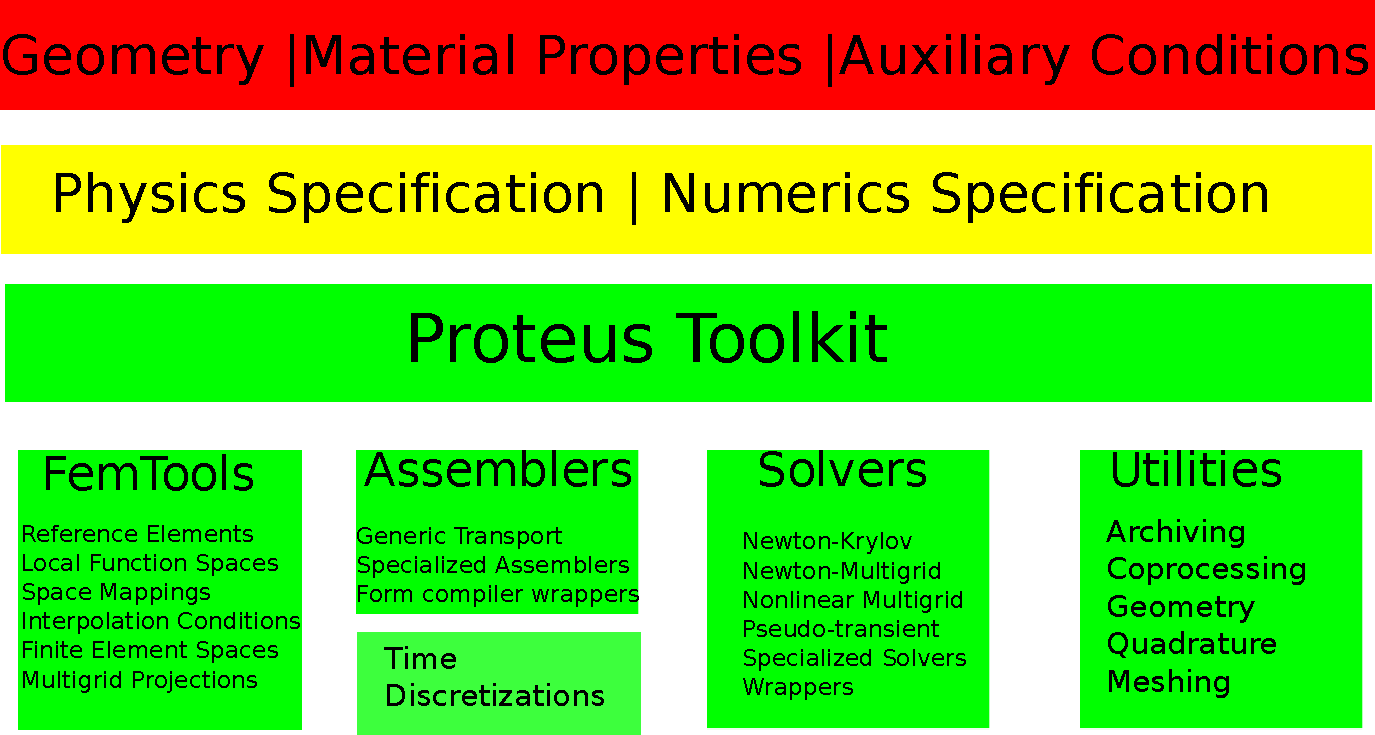
\includegraphics[scale=0.4]{modules.pdf}
\end{center}
\end{frame}


%5
\begin{frame}
\frametitle{Verified Numerics}
\bit
\footnotesize
\item Continuous linear and quadratic polynomial spaces ($C^0 P^1$ and $C^0 P^2$) on simplicial elements (intervals, triangles, tetrahedra) with nodal (Lagrange) basis
\item Continuous tensor product spaces ($C^0 Q^k$) on hexahedra with nodal basis
\item Discontinuous complete polynomial spaces ($C^{-1} P^k$) on simplicial elements with monomial basis
\item $P^1$ non-conforming simplicial elements (equivalent to Raviart-Thomas mixed element)
\item Eulerian-Lagrangian Localized Adjoint Methods (ELLAMs) for advection-dominated processes 
\item Locally discontinuous Galerkin mixed elements with static condensation
\item SIPG/NIPG/IIPG primal discontinuous elements
\item Residual-based variational multiscale methods (RBVMS)
\item Analytical Riemann solvers (numerical fluxes) for linear advection, two-phase flow in porous media, and shallow water
\item Approximate Riemann solvers: Harten-Lax-van Leer (SWE), Rusanov (two-phase flow), Cheng-Shu (Hamilton-Jacobi)
\item Velocity post-processing to enforce element-wise (local) conservation
\eit
\end{frame}

%6
\begin{frame}
  \frametitle{Verification and Validation Test Problems}
  \begin{minipage}{0.5\textwidth}
    \bit
  \item Dam break experiments
  \item Marin free surface flow/object experiment
  \item Wigley hull tow tank experiment
  \item Beach erosion board
  \item Flow around a cylinder
  \item Driven cavity
  \item Rotating Gaussian
  \item Advection in a vortex
  \item Porous media, slope stability,...
    %\item Poisseulle, Couette, and Decay of Vortex (low RE analytical solutions) 2D \& 3D
    \eit
  \end{minipage}\begin{minipage}{0.5\textwidth}
    \begin{overlayarea}{\textwidth}{\textwidth}
      \only<+>{\includemovie[controls,poster]{\textwidth}{\textwidth}{sloshbox2d.mov}}
      %      \only<+>{\includemovie[controls,poster]{\textwidth}{\textwidth}{dambreak2d.mov}}
      %      \only<+>{\includemovie[controls,poster]{\textwidth}{\textwidth}{sloshbox3d.mov}}
      \only<+>{\includemovie[controls,poster]{\textwidth}{\textwidth}{obstacle3d.mov}}
      %      \only<+>{\includemovie[controls,poster]{\textwidth}{\textwidth}{embankment.mov}}
    \end{overlayarea}
  \end{minipage}
\end{frame}

%7
\begin{frame}
\frt{Peer-Reviewed Verification and Validation}
\bit
\footnotesize
\item Implementation of Discontinuous Galerkin Methods for the
  Level-Set Equation on Unstructured Meshes, M. W. Farthing and C. E.
  Kees (2008) U.S. Army Engineer Research and Development Center,
  Coastal and Hydraulics Laboratory, Coastal and Hydraulics Technical
  Note, CHETN-XIII-2.

\item Locally conservative, stabilized finite element methods for
  variably saturated flow. C. E. Kees, M. W. Farthing, and C. N.
  Dawson (2008) {\em Computer Methods in Applied Mechanics and
    Engineering}, 197, 4610-4625.

\item Locally Conservative, Stabilized Finite Element Methods for a
  Class of Variable Coefficient Navier-Stokes Equations, C. E. Kees
  and M. W. Farthing (2009) ERDC-CHL TR-09-12.

\item A review of methods for moving boundary problems, C. E. Kees,
  M. W. Farthing, R. C. Berger, and T. C. Lackey (2009) ERDC-CHL
  TR-09-10.

\item Evaluating finite element methods for the level-set equation,
  M. W. Farthing and C. E. Kees (2009) ERDC-CHL TR-09-11.

\item A conservative level set method for variable-order
  approximations and unstructured meshes. C. E. Kees, I. Akkerman,
  M. W. Farthing, and Y. Bazilevs (2010) {\em Journal of Computational
    Physics}, In Press.
\eit
\end{frame}

%% \begin{frame}
%%   \frametitle{What is \textbf{petsc4py}?}  

%%   Python bindings for \textbf{PETSc}, the \emph{Portable Extensible
%%     Toolkit for Scientific Computation}.  
  
%%   \bigskip
 
%%   A \emph{good friend} of \textbf{petsc4py} is:
%%   \begin{itemize}
%%   \item \textbf{mpi4py}: Python bindings for \textbf{MPI}, the
%%     \emph{Message Passing Interface}.
%%   \end{itemize}
%%   \medskip
%%   Other two projects depend on petsc4py:
%%   \begin{itemize}
%%   \item \textbf{slepc4py}: Python bindings for \textbf{SLEPc}, the
%%     \emph{Scalable Library for Eigenvalue Problem Computations}.
%%   \item \textbf{tao4py}: Python bindings for \textbf{TAO}, the
%%     \emph{Toolkit for Advanced Optimization}.
%%   \end{itemize}
%% \end{frame}

%% \begin{frame}
%%   \frametitle{Implementation}
%%   Implemented with Cython \url{http://www.cython.org}
%%   \begin{itemize}
%%   \item Code base far easier to write, maintain, and extend.
%%   \item Faster than other solutions (mixed Python and C codes).
%%   \item Easier to cross language boundaries (reuse C/\Cpp/Fortran).
%%   \end{itemize}
%% \end{frame}

%% \begin{frame}
%%   \frametitle{Implementation - Cython [1]}
%%   \small\inputminted[firstline=1]{cython}{cython.pxi}
%% \end{frame}
%% \begin{frame}
%%   \frametitle{Implementation - Cython [2]}
%%   \small\inputminted[firstline=3]{cython}{cython.pyx}
%% \end{frame}

%% \begin{frame}
%%   \frametitle{Features -- PETSc components}
%%   \begin{itemize}
%%   \item \textbf{Index Sets}: permutations, indexing into vectors, renumbering.
%%   \item \textbf{Vectors}: sequential and distributed.
%%   \item \textbf{Matrices}: sequential and distributed, sparse and dense.
%%   \item \textbf{Distributed Arrays}: regular grid-based problems.
%%   \item \textbf{Linear Solvers}: Krylov subspace methods.
%%   \item \textbf{Preconditioners}: sparse direct solvers, multigrid
%%   \item \textbf{Nonlinear Solvers}: line search, trust region, matrix-free.
%%   \item \textbf{Timesteppers}: time-dependent, linear and nonlinear PDE's.
%%   \end{itemize}
%% \end{frame}

%% \begin{frame}
%%   \frametitle{Features -- Interoperability}
%%   Support for wrapping other PETSc-based codes.
%%   \begin{itemize}
%%   \item You can use \textbf{Cython} 
%%     (\texttt{from petsc4py {\bf cimport} PETSc}).
%%   \item You can use \textbf{SWIG} (\textsl{typemaps} provided).
%%   \item You can use \textbf{F2Py} (\texttt{fortran} attribute).
%%   \end{itemize}
%%   \bigskip
%%   (more on this later \ldots)
%% \end{frame}

%% \begin{frame}[fragile]
%%   \frametitle{Features -- Easy installation}
%% \begin{minted}{sh}
%% $ virtualenv --no-site-packages ENV
%% $ source ENV/bin/activate

%% (ENV) $ pip install slepc4py
%% Downloading/unpacking slepc4py
%% Downloading/unpacking petsc4py (from slepc4py)
%% Downloading/unpacking slepc (from slepc4py)
%% Downloading/unpacking petsc (from petsc4py->slepc4py)
%% Downloading/unpacking numpy (from petsc4py->slepc4py)
%% Installing collected packages: numpy, petsc, petsc4py,
%%                                slepc, slepc4py
%% (ENV) $
%% \end{minted}
%% \end{frame}

%% % --- Vectors & Matrices---

%% \section{Vectors \& Matrices}

%% \begin{frame}
%%   \frametitle{Vectors (\texttt{Vec}) -- Conjugate Gradients Method}
%%   \begin{columns}[t]
%%     \begin{column}{.45\textwidth}
%%       \tiny
%%       \begin{equation*}
%%         \begin{split}
%%           & cg(A,x,b,i_{max},\epsilon): \\
%%           & \quad i \Leftarrow 0 \\
%%           & \quad r \Leftarrow b - A x \\
%%           & \quad d \Leftarrow r \\
%%           & \quad \delta_{0} \Leftarrow r^T r \\
%%           & \quad \delta_{   } \Leftarrow \delta_{0} \\
%%           & \quad \text{while}\;\; i < i_{max} \text{ and } \\
%%           & \quad\quad\qquad  \delta_{   } > \delta_{0} \epsilon^2 \text{ do} :\\
%%           & \quad\quad\quad  q \Leftarrow Ad \\
%%           & \quad\quad\quad  \alpha \Leftarrow \frac{\delta_{   }}{d^T q} \\
%%           & \quad\quad\quad  x \Leftarrow x + \alpha d\\
%%           & \quad\quad\quad  r \Leftarrow r - \alpha q\\
%%           & \quad\quad\quad  \delta_{old} \Leftarrow \delta_{   } \\
%%           & \quad\quad\quad  \delta_{   } \Leftarrow r^T r \\
%%           & \quad\quad\quad  \beta \Leftarrow \frac{\delta_{   }}{\delta_{old}} \\
%%           & \quad\quad\quad  d \Leftarrow r + \beta d\\
%%           & \quad\quad\quad  i \Leftarrow i + 1
%%         \end{split}
%%       \end{equation*}
%%     \end{column}
%%     \begin{column}{.45\textwidth}
%%       \tiny\inputminted[linenos]{python}{petsc4py_vec.py}
%%     \end{column}
%%   \end{columns}
%% \end{frame}

%% \begin{frame}
%%   \frametitle{Matrices (\texttt{Mat}) [1]}
%%   \small\inputminted[linenos]{python}{petsc4py_mat_1.py}
%% \end{frame}

%% \begin{frame}
%%   \frametitle{Matrices (\texttt{Mat}) [2]}
%%   \small\inputminted[linenos]{python}{petsc4py_mat_2.py}
%% \end{frame}

%% % --- Linear Solvers  ---

%% \section{Linear Solvers}

%% \begin{frame}
%%   \frametitle{Linear Solvers (\texttt{KSP+PC})}
%%   \small\inputminted[linenos,firstline=3]{python}{petsc4py_ksp.py}
%% \end{frame}

%% % --- Nonlinear Solvers  ---

%% \section{Nonlinear Solvers}

%% \begin{frame}
%%   \frametitle{Nonlinear Solvers (\texttt{SNES}) [1]}
%%   \scriptsize\inputminted[linenos]{python}{petsc4py_snes_1.py}
%% \end{frame}

%% \begin{frame}
%%   \frametitle{Nonlinear Solvers (\texttt{SNES}) [2]}
%%   \small\inputminted[linenos]{python}{petsc4py_snes_2.py}
%% \end{frame}

%% % --- Interoperability ---

%% \section{Interoperability}

%% \begin{frame}
%%   \frametitle{Interoperability -- \textbf{Cython}}
%%   \scriptsize
%%   \inputminted[linenos]{cython}{wrap_cython.pyx}
%% \end{frame}

%% \begin{frame}
%%   \frametitle{Interoperability -- \textbf{SWIG}}
%%   \small
%%   \inputminted[linenos]{c}{wrap_swig.i}
%% \end{frame}

%% \begin{frame}
%%   \frametitle{Interoperability -- \textbf{F2Py}}
%%   \scriptsize
%%   \inputminted[linenos]{fortran}{wrap_f2py.pyf}
%% \end{frame}

%% % --- Performance ---

%% \section{Performance}

%% \newcommand{\onehalf}{\frac{1}{2}}
%% \newcommand{\pder}[2]{\ensuremath{\frac{\partial#1}{\partial#2}}}

%% \begin{frame}
%%   \frametitle{Performance}
%%   Consider the following diffusive, unsteady, non-linear, scalar
%%   problem in the unit cube $\Omega=(x,y,z)=(0,1)^3$
%%   \begin{itemize}
%%   \item PDE, boundary and initial conditions:
%%     \begin{equation}
%%       \begin{aligned}
%%         \pder{\phi}{t}-\nabla \cdot \left(\kappa(\phi)\nabla \phi \right) &= G
%%         ~~~\text{on $\Omega \times (0,T]$}\\
%%         \pder{\phi}{\mathbf{n}} &= 0 
%%         ~~~\text{at $\partial\Omega \times [0,T]$}\\
%%         \phi &= \phi^0
%%         ~~~\text{at $t=0$},
%%       \end{aligned}
%%     \end{equation}
%%   \item Nonlinear diffusion and line source term:
%%     \begin{equation} 
%%       \begin{aligned}
%%         \kappa(\phi)=
%%         \begin{cases}
%%           1 ~~~&\text{if } \phi \ge 0 \\
%%           \frac{1}{1+\phi^2} ~~~&\text{if } \phi < 0
%%         \end{cases}\\
%%         G(x=\dfrac{1}{4},y=\frac{1}{4},\frac{1}{2}<z<1) = -300
%%       \end{aligned}
%%     \end{equation}
%%   \end{itemize}
%% \end{frame}

%% \begin{frame}
%%   \frametitle{Performance --Discretization}
%% \begin{itemize}
%% \item finite differences in space
%% \item backward Euler in time
%% \end{itemize}
%% \vfill
%% \begin{equation}
%%   \frac{1}{\Delta t}(\phi^{n+1}_{i,j,k}-\phi^{n}_{i,j,k}) - 
%%   L_{i,j,k}(\kappa,\phi^{n+1}) - G_{i,j,k} = 0 
%% \end{equation}
%% \begin{equation}
%% \footnotesize
%% \begin{split}
%%     L_{i,j,k}(\kappa,\phi) = %\\
%%      &\frac{\kappa[i-\onehalf]}{(\Delta x_1)^2}                \phi[i-1]%
%%      -\frac{\kappa[i-\onehalf]+\kappa[i+\onehalf]}{(\Delta x_1)^2} \phi[0]%
%%      +\frac{\kappa[i+\onehalf]}{(\Delta x_1)^2}               \phi[i+1] +\\
%%     +&\frac{\kappa[j-\onehalf]}{(\Delta x_2)^2}               \phi[j-1]%
%%      -\frac{\kappa[j-\onehalf]+\kappa[j+\onehalf]}{(\Delta x_2)^2} \phi[0]%
%%      +\frac{\kappa[j+\onehalf]}{(\Delta x_2)^2}               \phi[j+1] +\\
%%     +&\frac{\kappa[k-\onehalf]}{(\Delta x_3)^2}               \phi[k-1]%
%%      -\frac{\kappa[k-\onehalf]+\kappa[k+\onehalf]}{(\Delta x_3)^2} \phi[0]%
%%      +\frac{\kappa[k+\onehalf]}{(\Delta x_3)^2}               \phi[k+1]
%% \end{split}
%% \end{equation}
%% (notation: %
%% $[0]=(i,j,k)$, $[i\pm\frac{1}{2}]=(i\pm\frac{1}{2},j,k)$, %
%% and so on)
%% \end{frame}

%% \begin{frame}
%%   \frametitle{Performance -- Python+F90 versus C+F90}
%%   Basically a measure of Python calling overhead \ldots
%%   \begin{itemize}
%%   \item equivalent Python and C codes for the drivers
%%   \item common Fortran 90 code for the nonlinear residual
%%   \item use matrix--free for the nonlinear problems
%%   \end{itemize}
%%   \begin{center}
%%     \includegraphics[scale=0.4]{petsc4py_oh.pdf}
%%   \end{center}
%% \end{frame}


%% % --- Closing ---

%% \section*{Closing}

%% \begin{frame}
%%   \Large
%%   Do not hesitate to ask for help \ldots 
%%   \bigskip
%%   \begin{itemize}
%%   \item Mailing List: \email{petsc-users@mcs.anl.gov}
%%   \item Mail\&Chat:   \email{dalcinl@gmail.com}
%%   \item Project Page: \url{http://petsc4py.googlecode.com}
%%   \end{itemize}
%%   \bigskip
%%   \begin{centering}
%%     \Huge Thanks!\par
%%   \end{centering}
%% \end{frame}

\end{document}


% Local Variables:
% mode: latex
% TeX-PDF-mode: t
% End:
